\documentclass{llncs}
%
\usepackage{makeidx}  % allows for indexgeneration

\usepackage[english]{babel}
\usepackage{amsmath,amssymb}
\usepackage{subfig}
\usepackage{graphicx}
\usepackage{tabularx}
\DeclareMathOperator{\sign}{sign}
\newcolumntype{K}[1]{>{\centering\arraybackslash}p{#1}}
%
\begin{document}
%
\mainmatter              % start of the contributions
%
\title{Parallel Multi-objective Optimization on CPU Using Information Framework for
Constructing Global Optimization Algorithms}
%
\titlerunning{Parallel Multi-objective Optimization}  % abbreviated title (for running head)
%                                     also used for the TOC unless
%                                     \toctitle is used
%
\author{Vladislav V. Sovrasov}
%
\authorrunning{Vladislav V. Sovrasov} % abbreviated author list (for running head)
%
%%%% list of authors for the TOC (use if author list has to be modified)
\tocauthor{Vladislav V. Sovrasov}
%
\institute{State University of Nizhny Novgorod, Nizhny Novgorod, Russia\\
\email{sovrasov.vlad@gmail.com}}

\maketitle              % typeset the title of the contribution

\begin{abstract}
In the present work, a parallel algorithm for the multi-objective optimization is considered. The
considered approach is based on the application of the information-statistical algorithm to some
reduced scalar problem, the set of the global optima in which coincides to the set of the
weakly efficient solutions of the initial multi-objective problem. The sequential version of this
method has been considered earlier. In the present work, the parallelization scheme based on
the characteristics, which is common for all information global search algorithms,
was applied to the sequential algorithm of the multi-objective optimization. Also, in the present
work one of the techniques of accounting for the local properties of the optimized function
allowing accelerating the convergence essentially has been considered for the multi-objective
method for the first time.

\keywords{deterministic global optimization, multi-objective optimization, parallel numerical
methods, derivative-free algorithms}
\end{abstract}
%
\section{Introduction}
The multi-objective optimization problems attract an increasing interest in recent years since
these ones reflect the controversy of the requirements arising to the modeled objects of real
world the most completely. In such problems, the solutions are a compromised decision of a set
of these ones. As a rule, these compromised solutions are chosen either from a set, in which all
elements cannot be improved with respect to any criterion without the worsening of the other
criteria (Pareto-optimal or efficient solutions) or from a set, in which no one element could be
improved with respect to all criteria at once (Slater-optimal or weakly efficient solutions). The
latter requirement is weaker, and all Pareto-optimal solutions are the Slater-optimal ones as
well.

To find the complete set of efficient or weakly efficient points is the most computationally
complex problem, however it provides a wide choice of possible compromised solutions. A
plenty of approaches to the finding of these sets has been developed: the application of the
genetic algorithms to the multi-objective problem directly~\cite{DebPratap2002}, the use of the
parametric convolutions reducing the problem to a series of the scalar global optimization
problems~\cite{GergelKozinov2017}, various approaches to the solving the problems with the
convex~\cite{ZhangZuo2013} or linear~\cite{Benson1998} objectives. The main problem in the
using of majority of these methods is the absence of the theoretical guarantee of the uniform
convergence to the whole sought set of the Pareto-optimal solutions on a wide class of
problems including the ones with the non-convex multiextremal criteria. A method having this
property in the case, when all criteria satisfy the Lipschitz condition has been developed on the
basis of the information global search algorithm~\cite{markinStrongin1993}. In the present
paper, the parallel and accelerated by the local refinement technique~\cite{strOptBook}(chapter
3) modification of this method will be considered.

\section{Problem Statement and Dimensionality Reduction}
The multi-objective optimization problems are stated in the following way:
\begin{equation}
  \label{eq:problem}
  \min\{f(y): y\in D\}, D=\{y\in \mathbb{R}^n: a_i \leqslant y_i \leqslant b_i, 1\leqslant i
\leqslant n \}
\end{equation}
Let us assume the components of the vector function (the partial criteria) \(f_i(y), 1\leqslant
i\leqslant m\) to satisfy the Lipschitz condition with the Lipschitz constant \(L_i\) in \(D\):
\begin{displaymath}
\label{lip}
|f_i(y_1)-f_i(y_2)|\leqslant L_i\Vert y_1-y_2\Vert,y_1,y_2\in D,0<L_i<\infty,1\leqslant i
\leqslant m
\end{displaymath}

The set \(S(D)\in D\) of strictly non-dominated points from the search domain is accepted as the
solution of the problem (\ref{eq:problem}) usually i. e.

\begin{equation}
  \label{eq:slater}
  S(D) = \{y\in D: \nexists z\in D, f_i(z)<f_i(y),1\leqslant i \leqslant m\}
\end{equation}

which is usually referred as the set of semi-efficient (or weakly efficient) solutions. The
conditions in the right-hand side of the definition (\ref{eq:slater}) are known as the principle of
weak Pareto-optimality (or Slater's optimality principle).

The use of the evolvents \(y(x)\) i. e. the space-filling curves is a classic dimensionality
reduction scheme for global optimization algorithms~\cite{evolvents2013}.
\begin{displaymath}
\label{cube}
\lbrace y\in R^N:-2^{-1}\leqslant y_i\leqslant 2^{-1},1\leqslant i\leqslant
N\rbrace=\{y(x):0\leqslant x\leqslant 1\}
\end{displaymath}
\par
Such a mapping allows the reduction of the problem (\(\ref{eq:problem}\)) stated in a
multidimensional space to solving a one-dimensional problem at the expense of worsening its
properties.
In particular, the one-dimensional functions \(f_i(y(x))\) are not Lipschitzian but the
H\"olderian functions:
\begin{equation}
\label{eq:holder}
|f_i(y(x_1))-f_i(y(x_2))|\leqslant H_i{|x_1-x_2|}^{\frac{1}{N}},x_1,x_2\in[0,1]
\end{equation}
where the H\"older constants \(H_i\) are related to the Lipschitz constant \(L_i\) by the relation
\begin{displaymath}
H_i=4L_id\sqrt{N},d=\max\{b_i-a_i:1\leqslant i\leqslant n\}
\end{displaymath}
\par
Therefore, not limiting the generality, one can consider the solving of the
one-dimensional problem \(\min\{f(y(x)): x\in [0;1]\}\), satisfying the H\"older condition. The
issues of the numerical building the mapping like a Peano curve and the corresponding theory
have been considered in detail in~\cite{evolvents2013}. Here we would note that an evolvent
built numerically is an approximation of the theoretical Peano curve with a precision of the
order \(2^{-m}\) where \(m\) is the building parameter of the evolvent.

\section{Description of the Parallel Algorithm With Local Refinement}
\label{sec:algorithm}
Let us consider a scalarization scheme for the reduced problem (\(\ref{eq:problem}\)),
presented in~\cite{markinStrongin1993}. Let
\begin{equation}
  \varphi(x)=\max\{h(x,y):y\in [0;1]\},x\in [0;1].
\end{equation}
Let us consider a scalar problem
\begin{equation}
  \label{eq:aux_problem}
  \varphi^*=\min\{\varphi(x):x\in [0;1]\}.
\end{equation}

As it has been shown in~\cite{markinStrongin1993}, the set of weakly efficient solutions of the
reduced problem (\ref{eq:problem}) coincides to the set of the globally optimal solutions of
the problem (\ref{eq:aux_problem}) i. e.
\begin{equation}
  \label{eq:s}
  S([0;1])=\{x\in [0;1]:\varphi(x)=\varphi^*\}
\end{equation}
Also, it has been shown in~\cite{markinStrongin1993} that the function \(\varphi(x)\) satisfies
the H\"older condition when the requirements (\ref{eq:holder}) are satisfied. Thus, the
information-statistical global search algorithm can be applied to the function \(\varphi(x)\) in
order to solve the problem (\ref{eq:aux_problem}). However, \(\varphi(x)\) is defined through
the operator \(\max\{...\}\), therefore, it is difficult to compute it directly. In
\cite{markinStrongin1993}, a modification of the classic information
global search algorithm~\cite{mixedAlg} is given, in which the values of \(\varphi(x)\) are computed
approximately. Let us consider the modified version of this algorithm. The modification
consists in the use of the local refinement technique described in~\cite{strOptBook}(chapter 3)
as well as in the parallelization based on the characteristics~\cite{strOptBook}(chapter 5).

The first two iterations are performed at the boundary points~\(x^0=0\) and \(x^1=1\) of the
interval \([0;1]\). The choice of the points \(x^{k+j}, 1\leqslant j\leqslant p\) is performed
according to the following rules:

\textit{Step 1.} Renumber the points in the set \(X_k=\{x^1,\dotsc,x^k\}\cup\{0\}\cup\{1\}\),
which includes the boundary points of the interval \([0,1]\) as well as the points of preceding
trials, by the lower indices in order of increasing coordinate values  i. e.
\begin{displaymath}
  0=x_0<x_1<\dotsc<x_{k+1}=1
\end{displaymath}

\textit{Step 2.} Compute the lover bound \(\mu_\nu\) for the Lipzhitz constant for each
objective function \(f_\nu(x),1\leqslant\nu\leqslant m\):
\begin{gather}
\label{eq:step2_1}
\mu_\nu=\max_{1\leqslant i\leqslant k}\dfrac{|f_\nu(x_i)-f_\nu(x_{i-1})|}{\Delta_i}, 1\leqslant
\nu\leqslant m \\
\label{eq:step2_2}
\Delta_i=(x_i-x_{i-1})^\frac{1}{N}
\end{gather}

\textit{Step 3.} To each point \(x_i\), \(0\leqslant i\leqslant k\), juxtapose the value
\begin{equation}
  z_i=\max\{h(x_i,x_j):0\leqslant j\leqslant k\},
\end{equation}
where
\begin{equation}
  h(x_i,x_j)=\min\{\frac{f_\nu(x_i)-f_\nu(x_j)}{\mu_\nu}:1\leqslant \nu\leqslant m\}, 0\leqslant
i,j\leqslant k
\end{equation}

\textit{Step 4.} For each interval \((x_i,x_{i-1}),1\leqslant i\leqslant k\) compute two
characteristics:
\begin{eqnarray}
  R(i) = \Delta_i + \frac{(z_i-z_{i-1})^2}{r^2\Delta_i}-\frac{z_i+z_{i-1}}{2r} \\
  R^*(i)=\frac{R(i)}{\sqrt{(z_i-z^*)(z_{i-1}-z^*)} + 1.5^{-\alpha}},
\end{eqnarray}
where \(\Delta_i\) is from (\ref{eq:step2_2}), \(z^*=\min\{z_i:1\leqslant i\leqslant k\}\). \(r>1\),
and \(\alpha\in [10;30]\) are the input parameters of the algorithm.

\textit{Step 5.} If \(q\not=0\) and \(s \mod q\not=0 \), then arrange the characteristics \(R(i)\),
\(1 \leqslant i \leqslant k + 1\) in the decreasing order
\begin{equation*}
  R(t_1) \geqslant R(t_2) \geqslant \dots \geqslant R(t_k) \geqslant R(t_{k+1})
\end{equation*}
and select \(p\) maximum characteristics with the indices of the intervals \(t_j\), \(1 \leqslant j
\leqslant p\). Otherwise do the same with the characteristics \(R^*(i),1\leqslant i\leqslant k+1\).
Here \(s\) is the index of current iteration and \(q\) is the parameter of the method responsible
for the degree of intensity of the local refinement. The less \(q\), the more frequent the
characteristics \(R^*\) are used making the method to choose the next points near the current
minimum found.

\textit{Step 6.} Perform the new trials at the points \(x^{k+j}\), \(1 \leqslant j \leqslant p\):
\begin{equation}
  x^{k+j}=\frac{x_{t_j}+x_{t_j-1}}{2} - \sign(z_{t_j} - z_{t_j-1})\frac{|z_{t_j} - z_{t_j-
1}|^n}{2r}
\end{equation}
All \(p\) trials within this step can be performed in parallel on \(p\) computing devices.

The algorithm is terminated if the condition \(\Delta_{t_j}\leqslant \varepsilon\) is fulfilled at
least for one of the indices \(t_j\), \(1\leqslant j\leqslant p\); here \(\varepsilon >0\) is the
predefined accuracy.
After the search is terminated, the set \(S(\{x^0,\dots ,x^k\})\) of all
non-dominated points of the truncated sequence \(\{x^0,\dots ,x^k\}\) is accepted as an
estimation for \(S\) from (\ref{eq:s}).

The theoretical substantiation of this method when \(p=1\) and \(q=0\) is presented in
\cite{strOptBook}(chapter 3). The siffitient condition of convergence is: there exists an
iteration such that \(r\mu_\nu \geqslant 4H_\nu, 1\leqslant \nu \leqslant m\).
\section{Test Problems}
\label{sec:test_problems}
In order to evaluate the degree of speedup of the convergence of the modified algorithm from
Section \ref{sec:algorithm}, the following problems were used:
\begin{enumerate}
  \item Markin-Strongin problem from \cite{markinStrongin1993}:
    \begin{equation}
      \left \{
      \begin{array}{l}
        f_1(y) = \min\{\sqrt{y_1^2+y_2^2},\sqrt{(y_1-1.5)^2+(y_2+1.5)^2}\} \\
        f_2(y)=\sqrt{(y_1+0.5)^2+(y_2-0.5)^2} \\
      \end{array}
      \right .
      y_1\in [-1;2],y_2\in [-2;1]
    \end{equation}
  \item Fonseca and Fleming problem \cite{Huband2006}:
  \begin{equation}
    \label{eq:fonseca}
    \left \{
    \begin{array}{l}
      f_{1}\left(y\right) = 1 - \exp \left(-\sum_{i=1}^{n} \left(y_{i} - \frac{1}{\sqrt{n}}
\right)^{2} \right) \\
      f_{2}\left(y\right) = 1 - \exp \left(-\sum_{i=1}^{n} \left(y_{i} + \frac{1}{\sqrt{n}}
\right)^{2} \right) \\
    \end{array}
    \right .
    \quad y\in [-4;4]^n
  \end{equation}
  \item
  Viennet function
  \begin{equation}
    \left \{
    \begin{array}{l}
      f_{1}\left(y\right) = 0.5(y_1^2 + y_2^2) + \sin(y_1^2 + y_2^2)\\
      f_{2}\left(y\right) = \frac{(3y_1 - 2y_2 + 4)^2}{8} + \frac{(y_1-y_2 + 1)^2}{27} + 15\\
      f_{3}\left(y\right) = \frac{1}{y_1^2+y_2^2 + 1} -1.1 \exp\{-(y_1^2+y_2^2)\}\\
    \end{array}
    \right .
    \quad y\in [-3;3]^2
  \end{equation}
%  Schaffer function N. 2 \cite{Huband2006}:
%    \begin{equation}
%      \label{eq:schaffer2}
%      \left \{
%      \begin{array}{l}
%        f_1(y) = \begin{cases}
%                  -y,   & \text{if } y \leqslant 1 \\
%                   y-2, & \text{if } 1 < y \leqslant 3 \\
%                   4-y, & \text{if } 3 < y \leqslant 4 \\
%                   y-4, & \text{if } y > 4 \\
%                \end{cases} \\
%        f_2(y) = (y-5)^2\\
%      \end{array}
%      \right .
%      \quad y\in [-5;10]
%    \end{equation}
  \item Poloni's two objective function \cite{Huband2006}:
    \begin{equation}
      \left \{
      \begin{array}{l}
        f_{1}\left(y\right) = \left[1 + \left(A_{1} - B_{1}\left(y\right) \right)^{2} + \left(A_{2} -
B_{2}\left(y\right) \right)^{2} \right] \\
        f_{2}\left(y\right) = \left(y_1 + 3\right)^{2} + \left(y_2 + 1 \right)^{2} \\
      \end{array}
      \right .
      \quad y\in [-\pi;\pi]^2
    \end{equation}
    where
    \begin{equation*}
      \begin{cases}
        A_{1} = 0.5 \sin \left(1\right) - 2 \cos \left(1\right) + \sin \left(2\right) - 1.5 \cos
\left(2\right)  \\
        A_{2} = 1.5 \sin \left(1\right) - \cos \left(1\right) + 2 \sin \left(2\right) - 0.5 \cos
\left(2\right)  \\
        B_{1}\left(y\right) = 0.5 \sin \left(y_1\right) - 2 \cos \left(y_1\right) + \sin \left(y_2\right) -
1.5 \cos \left(y_2\right)  \\
        B_{2}\left(y\right) = 1.5 \sin \left(y_1\right) - \cos \left(y_1\right) + 2 \sin \left(y_2\right) -
0.5 \cos \left(y_2\right)
      \end{cases}
    \end{equation*}
%  \item A problem considered in \cite{}:
%    \begin{equation}
%      \left \{
%      \begin{array}{l}
%        f_1(y) = (y_1 - 1)y_2^2 +1 \\
%        f_2(y)= y_2 \\
%      \end{array}
%      \right .
%      \quad y\in [0;1]^2
%    \end{equation}
\end{enumerate}
\section{Experimental Results}
The computational experiments have been carried out on the Lobachevsky supercomputer at
Lobachevsky State University of Nizhni Novgorod. A computational node included 2 Intel
Sandy Bridge E5-2660 2.2 GHz processors, 64 Gb RAM. The CPUs had 8 cores (i. e. total 16 cores
were available per a node).
In the present section, we will understand the speedup of the method as the speedup in the
number of executed iterations, not in the time of execution. If the computation of the problem
criteria (\ref{eq:problem}) takes enough much time, the overhead costs for the execution of the
decision rules of the optimization method are low as compared to the time of computing the
criteria \(f_i(y), 1\leqslant i\leqslant m\).

\paragraph{Local refinement advantages.} In \cite{barkalovLebedev2016} the numerical
experiments demonstrating the speedup of convergence when using the local refinement
technique in the algorithm solving the scalar global optimization problems are presented. One
could expect similar results from the multi-objective algorithm as well. The multi-objective
algorithm with local refinement (MOALR) has been applied to the  Fonseca and Fleming
problem (\ref{eq:fonseca}) at \(n=2\). The parameters of the method were as follows:
\(\varepsilon=0.01,\;r=4,\;q=4,\;\alpha=15,\;p=1\). Before the method stops, 1176 iterations
have been executed, the number of found weakly optimal points was 90. At \(q=0\) (without the
local refinement) the method had performed 1484 iterations, the number of found weakly
optimal points was 93. In fig. \ref{fig:fonseca_slater} the set \(S\) in the problem
(\ref{eq:fonseca}) and the numerical estimates of this one obtained at \(q=0\) (fig.
\ref{fig:fonseca_slater}.a) and \(q=4\) (fig. \ref{fig:fonseca_slater}.b) are presented. It is
evident also from fig. \ref{fig:fonseca_slater} that the approximate solution covers the whole
set of the weak-optimal solutions.

\begin{figure}[ht]
    \centering
    \subfloat[MOALR with
\(q=0\)]{{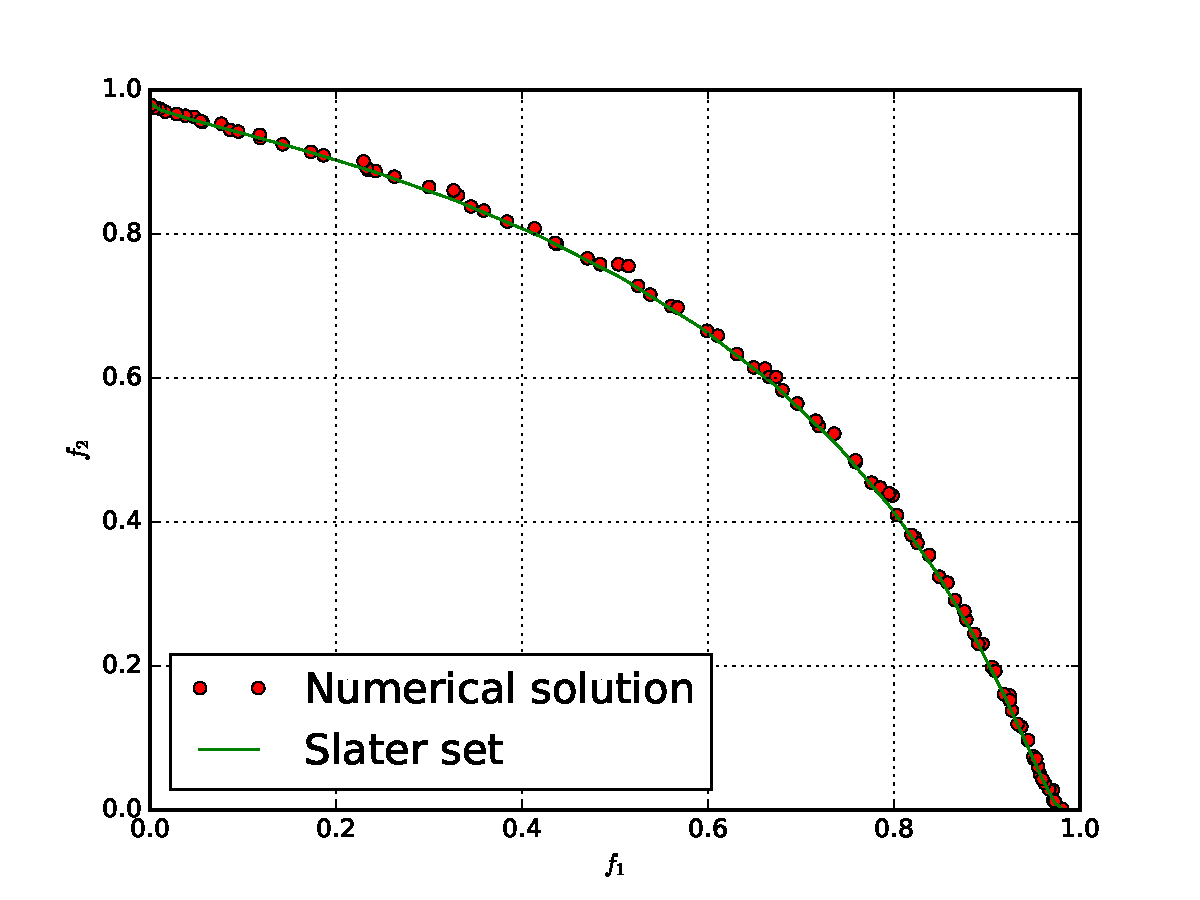
\includegraphics[width=.5\textwidth]{img/fonseca_glob.pdf} }}
    \subfloat[MOALR with
\(q=4\)]{{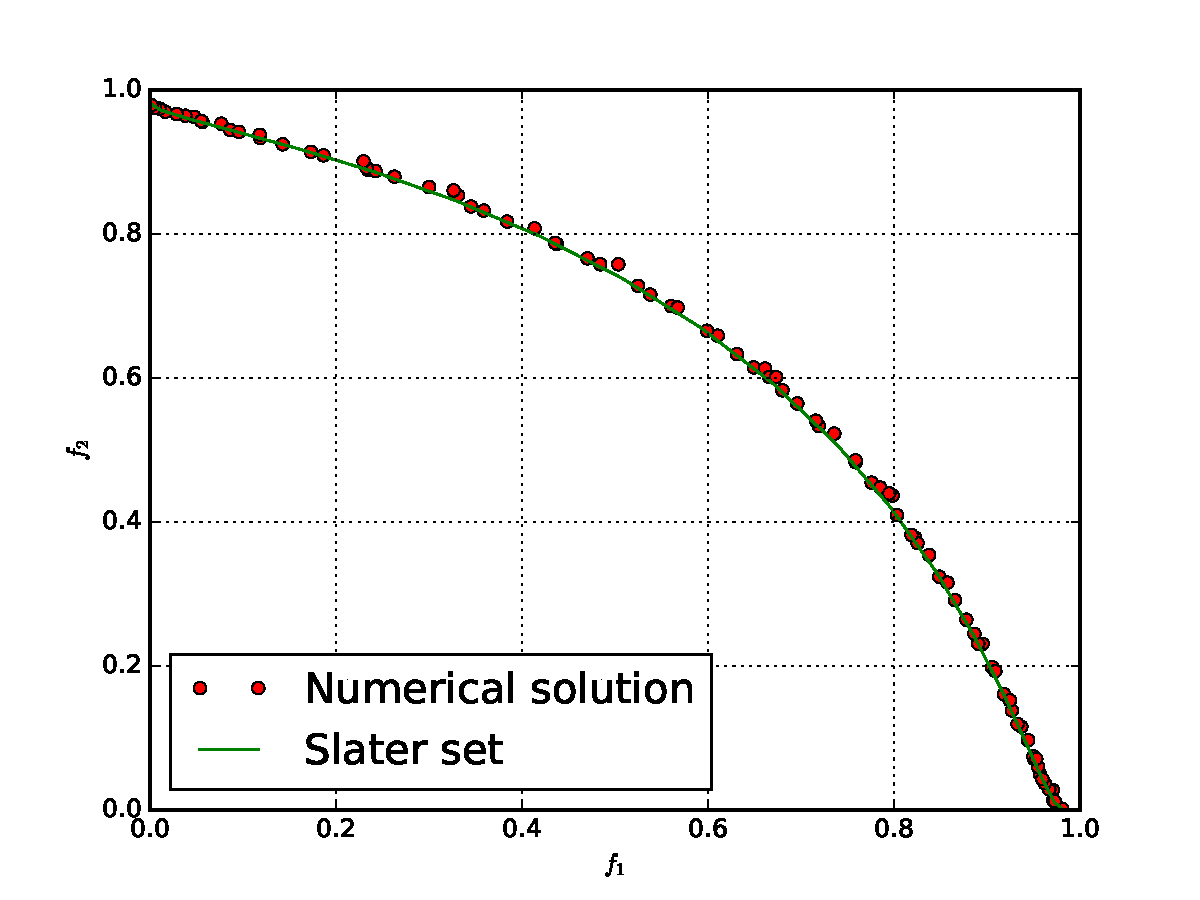
\includegraphics[width=.5\textwidth]{img/fonseca_loc.pdf} }}
    \caption{Numericas estimation of \(S\) obtained by MOALR}
    \label{fig:fonseca_slater}
\end{figure}

Below, MOALR with \(q=4\) was used for all experiments.

\paragraph{Parallel method results.} In order to demonstrate the speedup in iterations, which
MOALR provides when \(p > 1\), all problems from Section \ref{sec:test_problems} have been
solved for the values \(p=1,2,4,8,16\). The parameres of the method were the following:
\(r=4.5\), \(\varepsilon=0.01\), \(\alpha=15\). The number of iterations is presented in Table \ref{tab:exResultsIters}
(in the braces, the cardinalityof the set \(S\) is given) and the speedup in iterations is presented
in in Table \ref{tab:exResultsItersSpeedup}. As it is evident form Table
\ref{tab:exResultsIters}, the cardinality of the set \(S\) changed insuffiliently when varying \(p\)
i. e. the quality of the obtained estimates remained the same. At the same time, the number of
iterations decreased linearly with increasing value of \(p\) (Table
\ref{tab:exResultsItersSpeedup}). In fig. \ref{fig:s_estimation_all}, the examples of the
numerical solutions of the considered problems are given.

\begin{table}
  \centering
  \caption{Results of numerical experiments: number of iterations}
  \label{tab:exResultsIters}
  \begin{tabular}{|l|K{1.7cm}|K{1.7cm}|K{1.7cm}|K{1.7cm}|K{1.7cm}|}
\hline
\textbf{Problem} & \multicolumn{5}{c|}{\(p\)}\\
\cline{2-6}
  & \(1\) & \(2\) & \(4\) & \(8\) & \(16\)\\
\hline
Markin-Strongin & 1041(198) & 516(198) & 256(185) & 131(197) & 68(191) \\
\hline
Fonseca and Fleming 2d & 1181(93) & 636(99) & 386(111) & 176(95) & 106(97) \\
\hline
Fonseca and Fleming 3d & 5346(160) & 3551(183) & 1186(143) & 606(153) & 351(142) \\
\hline
Viennet problem & 4896(276) & 2156(273) & 1226(270) & 631(287) & 286(274)\\
\hline
Poloni's function & 3351(102) & 1706(90) & 856(88) & 426(96) & 201(99) \\
\hline
\end{tabular}
\end{table}

\begin{table}
  \centering
  \caption{Results of numerical experiments: speedup in iterations}
  \label{tab:exResultsItersSpeedup}
  \begin{tabular}{|l|K{1.5cm}|K{1.5cm}|K{1.5cm}|K{1.5cm}|}
\hline
\textbf{Problem} & \multicolumn{4}{c|}{\(p\)}\\
\cline{2-5}
  & \(2\) & \(4\) & \(8\) & \(16\)\\
\hline
Markin-Strongin & 2.02 & 4.07 & 7.95 & 15.31 \\
\hline
Fonseca and Fleming 2d & 1.86 & 3.06 & 6.71 & 11.14 \\
\hline
Fonseca and Fleming 3d & 1.51 & 4.51 & 8.82 & 15.23 \\
\hline
Viennet problem & 2.27 & 3.99 & 7.76 & 17.12\\
\hline
Poloni's problem & 1.96 & 3.91 & 7.87 & 16.67 \\
\hline
\end{tabular}
\end{table}

\begin{figure}[ht]
    \centering
    \subfloat[Markin-Strongin
problem]{{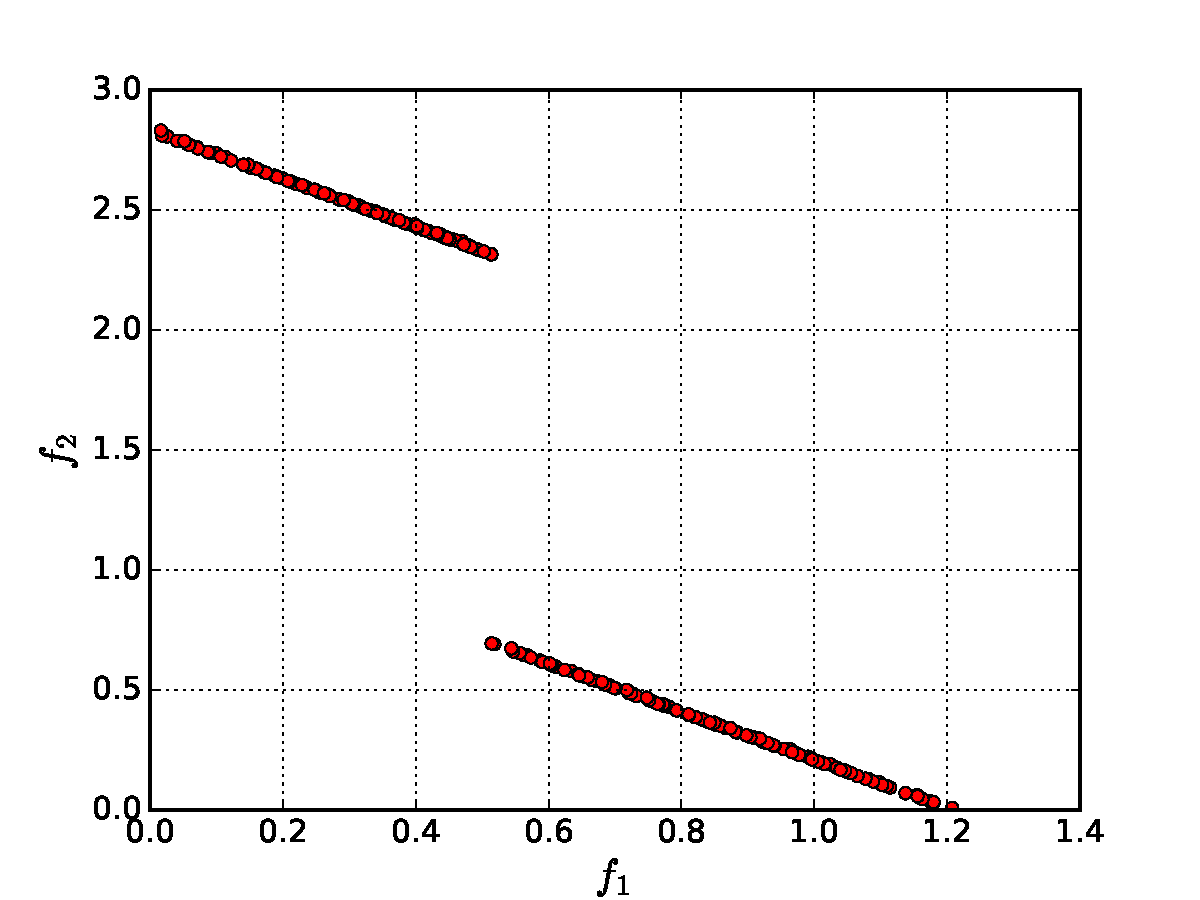
\includegraphics[width=.5\textwidth]{img/strongin.pdf} }}
    \subfloat[Fonseca and Fleming 3d
problem]{{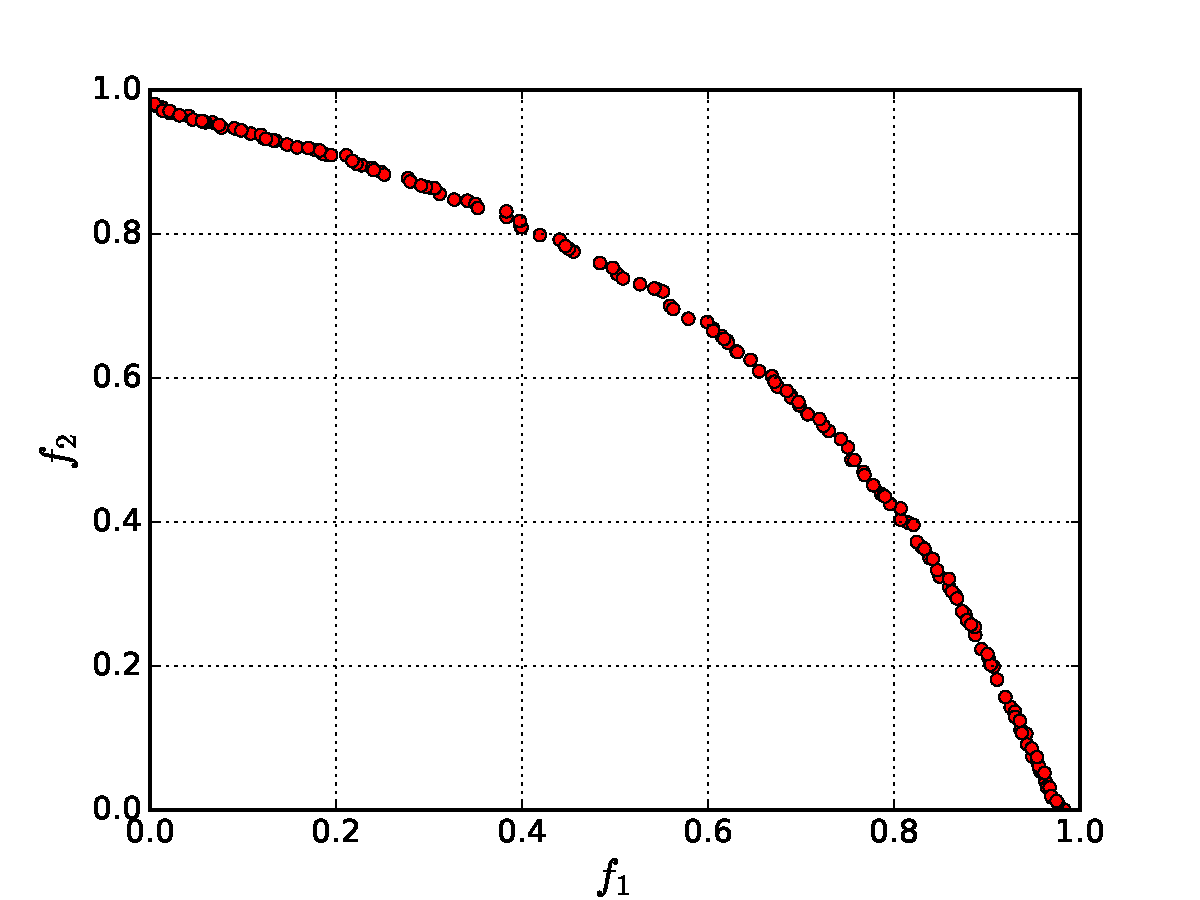
\includegraphics[width=.5\textwidth]{img/fonseca.pdf} }}

    \subfloat[Viennet problem]{{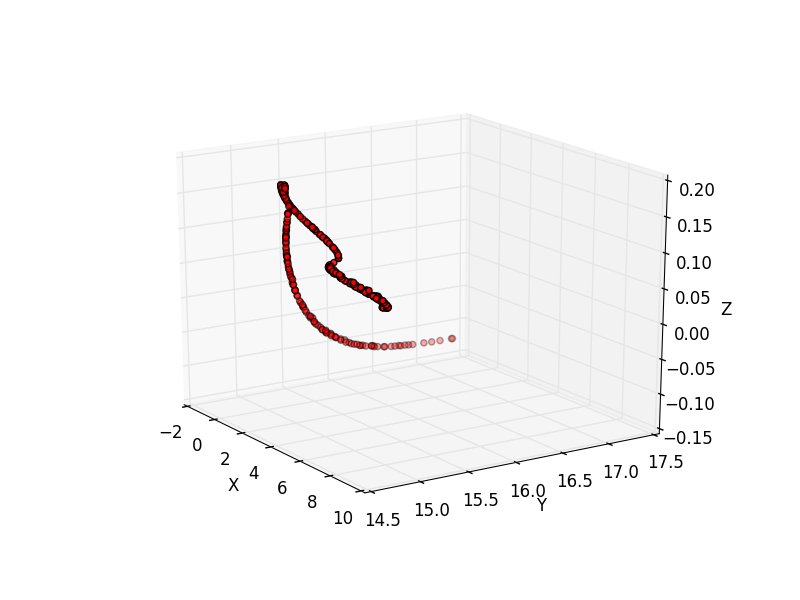
\includegraphics[width=.5\textwidth]{img/viennet.png}
}}
    \subfloat[Poloni's problem]{{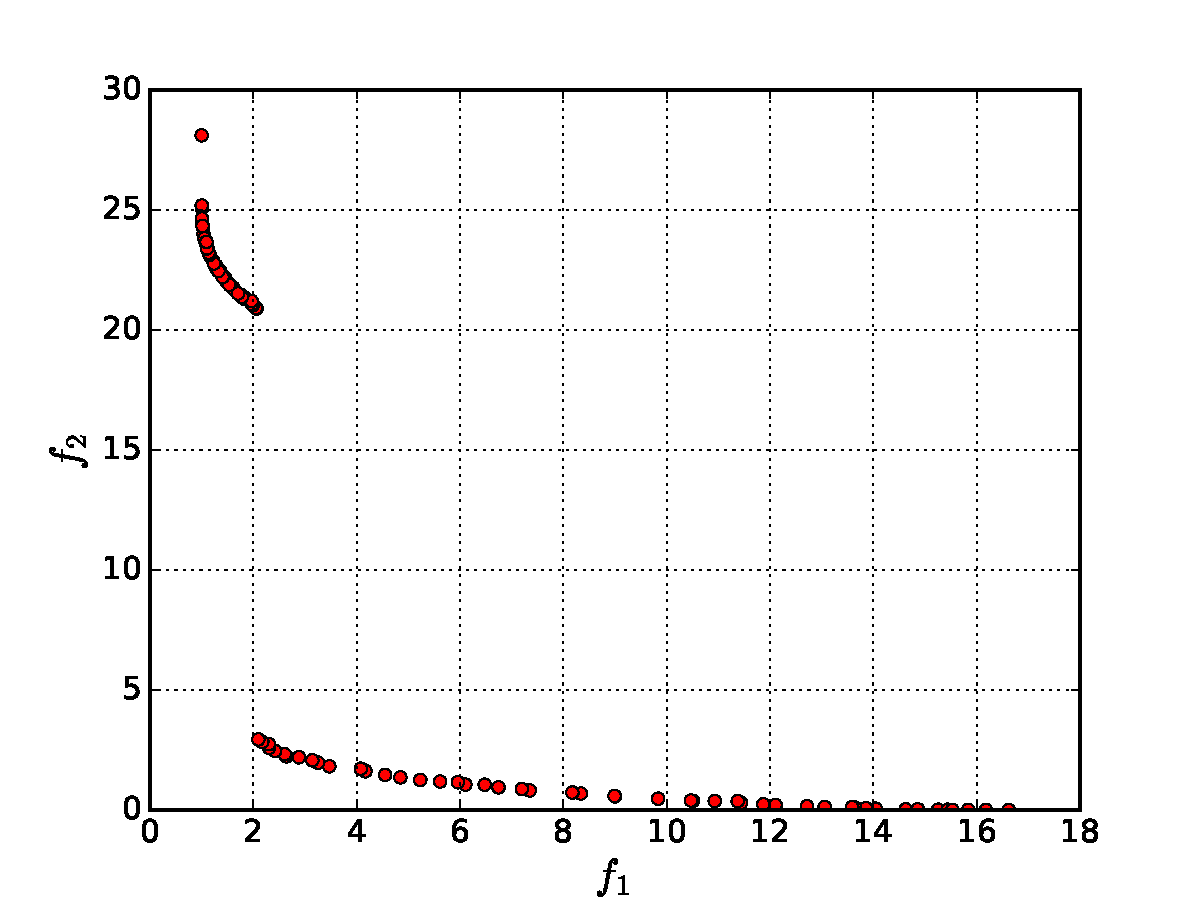
\includegraphics[width=.5\textwidth]{img/poloni.pdf} }}
    \caption{Numericas estimations of \(S\) obtained by MOALR}
    \label{fig:s_estimation_all}
\end{figure}

\paragraph{Parallel method time speedup.} The objective functions of all problems listed in this
section are featured by low computational complexity. In order to demonstrate the possibility to
obtain a speedup in time for the problems with the hard-to-compute criteria, additinal intensive
froating point computations not affecting the resulting values were introduced into the criteria.
The speedups obtained are given in Table \ref{tab:exResultsTimeSpeedup}. In all cases, the
speedup in time was less than the speedip in iterations because the operation of the optimizaion
method itself takes a part of the execution time. However, in most cases the parallelizaion was
efficient enough even in the case of 16 CPU threads. For more computation costly criteria, one can
expect the increasing of the speedup in time for a large number of threads.

\begin{table}[ht]
  \centering
  \caption{Results of numerical experiments: speedup in time}
  \label{tab:exResultsTimeSpeedup}
  \begin{tabular}{|l|K{1.5cm}|K{1.5cm}|K{1.5cm}|K{1.5cm}|K{1.5cm}|}
\hline
\textbf{Problem} & \multicolumn{5}{c|}{\(p\)}\\
\cline{2-6}
&\(1\)(time, s) & \(2\) & \(4\) & \(8\) & \(16\)\\
\hline
Markin-Strongin & 104.47 & 1.97 & 3.65 & 6.79 & 9.90 \\
\hline
Fonseca and Fleming 2d & 118.95 & 1.85 & 2.81 & 5.79 & 6.40 \\
\hline
Fonseca and Fleming 3d & 554.45 & 1.51 & 4.14 & 8.05 & 10.69 \\
\hline
Viennet problem & TBD & TBD & TBD & TBD & TBD\\
\hline
Poloni's problem & 336.74 & 1.82 & 3.64 & 6.98 & 10.60 \\
\hline
\end{tabular}
\end{table}

\section{Conclusion}
In the present work, a method for solving the multi-objective optimizaion problems allowing
finding a uniform estimate of the set of the weakly-optimal points has been considered. The
techniques of parallelization and of the acceleration of convergence common for all algorithms
of similar structure have been applied. The numerical experiments performed have
demonstrated a speedup in convergence when using the local refinement. Also, the
parallelization based on the characteristics was found to be efficient for this method. The
speedup in iterations at the parallelization based on the characteristics appeared to be linear in
most cases as for the information methods of scalar optimization (see the results of the
parlallelization of the scalar optimization method, for example, in
\cite{barkalovLebedef2016}). From the results of the experiments, one can conclude that it is
expedient to apply sthe parallel MOALR in the problems of low dimensionality (1 to 3) with
the computation-costly criteria. Besides, the property of uniform convergence of the considered
algorithm to the whole set of the weakly-optimal solutions has been demonstrated on the
numerical examples.
%
% ---- Bibliography ----
%
%\bibliographystyle{plain}
%\bibliographystyle{alpha}
\bibliographystyle{unsrt}
%\bibliographystyle{splncs03}
\bibliography{u_pdc_refs}

\clearpage
\addtocmark[2]{Author Index} % additional numbered TOC entry
\renewcommand{\indexname}{Author Index}
\printindex
\clearpage
\end{document}
